%%%%%%%%%%%%%%%%%%%%%%%%%%%%%%%%%%%%%%%%%%%%%%%%%%%%%%%%%%%%%%%%%%%%%%%%%%%%%%%%%%%%%%%%%%%%%%%%%%%%%%%%%%%%%%%%%%%%%%%%%%%%%%%%%%%%%%%%%%%%%%%%%%%%%%%%%%%%%%%%%%%%%%%
%%%%%%%%%%%%%%%%%%%%%%%%%%%%%%%%%%%%%%%%%%%%%%%%%%%%%%%%%%%%%%%%%%%%%%%%%%%%%%%%%%%%%%%%%%%%%%%%%%%%%%%%%%%%%%%%%%%%%%%%%%%%%%%%%%%%%%%%%%%%%%%%%%%%%%%%%%%%%%%%%%%%%%%
\FloatBarrier
\chapter{Optimisation of the search sensitivity}
\label{ch:Optimisation}
Finally, having all background estimation methods in place, an optimisation procedure is conducted in order to increase the search sensitivity with respect to different signal models as introduced in Section~\ref{sec:SignalSamples}.
The optimisation is done in the most sensitive variables, \pt and \ias (see Section~\ref{sec:Ias} for a definition and explanation of the Asymmetric Smirnov discriminator \ias).
A potential additional discriminating variable is the number of missing outer hits \nlostouter in the tracker system. 
This variable is, however, not considered in this analysis because the discriminating potential for this search is limited, as shown in Appendix~\ref{app:OptimisationNLostOuter}.\\

SUSY models with different chargino lifetimes and masses are characterised by different \pt and \ias distributions as well as different theoretical cross sections.
Therefore, the usual search optimisation strategy that maximises $N_S/\Delta B$ ($N_S$ = number of signal events of model $S$, $\Delta B$ = background uncertainty) implies a potential fine-tuning on the specific SUSY cross sections.
In order to keep the search as general as possible, a cross section independent optimisation is performed.
This is achieved by a minimisation of the cross section for which a 5$\sigma$-discovery ($\kappa=5$) of the corresponding signal model is expected, \ie finding the optimal selection cuts for \pt and \ias for which the lowest possible cross section, $\sigma_{\text{min}}$, can be discovered
\begin{align}
\label{eq:optimisation}
%\frac{\sigma_{\text{min}}\cdot \mathcal{L}}{\Delta B} = \frac{\sigma_{\text{min}}\cdot \mathcal{L}}{\sqrt{ \left(\Delta B_{\text{stat}}\right)^2 + \left(\Delta B_{\text{sys}}\right)^2}} \geq 5.
\kappa = \frac{\alpha_{\text{min}} \cdot N_S(\text{mass},\ctau,\pt^{\text{cut}}, \ias^{\text{cut}})}{\Delta B (\pt^{\text{cut}}, \ias^{\text{cut}})} = 5. && \text{with   } \alpha_{\text{min}} = \frac{\sigma_{\text{min}}}{\sigma_{S}}.
\end{align}
The number of expected events $N_S$ of the signal model $S$ depends on the \pt and \ias selection cut as well as the mass and the lifetime of the chargino.
The uncertainty on the background $\Delta B$ is dependent on the \pt and \ias cut, and takes into account the full systematic uncertainty as well as the statistical uncertainty on the background prediction which is defined as the 68\% one sided upper limit of a Poisson distribution with $\mu = N_B$ estimated with the Neyman construction~\cite{bib:Neyman_1937,bib:PDG_2014}.
The systematic uncertainty on the background prediction includes systematic uncertainties as described in Section~\ref{sec:SysUncertaintiesBkg}, and statistical uncertainties arising from limited statistical precision of the control regions and simulated samples used in the background estimation.
The factor $\alpha_{\text{min}}$  that is minimised is the ratio of the minimum cross section $\sigma_{\text{min}}$ divided by the nominal cross section $\sigma_{S}$ of the signal model S.\\

As this analysis focuses on short tracks, rather low lifetimes are considered in the optimisation procedure: $\ctau=1\cm,\,10\cm,\,50\cm$.
These lifetimes are further suitable as they lie at the edge of the sensitivity of the search for disappearing tracks~\cite{bib:CMS:DT_8TeV}.
To cover the full mass space, the optimisation is done for masses between 100\gev and 500\gev in steps of 100\gev.

The corresponding results are shown in Table~\ref{tab:optimisation}.
\renewcommand{\arraystretch}{1.5}
\begin{table}[!h]
\centering
\caption{Optimal \pt and \ias selection cuts and the corresponding minimum cross section $\sigma_{\text{min}}$ that can be discovered with 5$\sigma$ significance for different signal models.
         For some signal samples, an optimisation result is not available due to the limited size of these samples.}
\label{tab:optimisation}
\makebox[0.99\textwidth]{
\begin{tabular}{c |c| c| c| c}
\multicolumn{5}{c}{} \\
\toprule
Mass [\gev] & Lifetime [\cm] & Optimal \pt cut & Optimal \ias cut & $\sigma_{\text{min}}$ \\
\midrule
100&                     1&                       30&                      0.05&                    61.596\\
200&                     1&                       20&                      0.05&                    43.414\\
300&                     1&                       n/a &                    n/a &                    n/a \\  
400&                     1&                       n/a &                    n/a &                    n/a \\  
500&                     1&                       n/a &                    n/a &                    n/a \\  
\midrule
100&                     10&                      30&                      0.05&                    1.531\\ 
200&                     10&                      30&                      0.30&                    0.561\\ 
300&                     10&                      30&                      0.30&                    0.354\\ 
400&                     10&                      30&                      0.30&                    0.238\\ 
500&                     10&                      50&                      0.30&                    0.201\\ 
\midrule
100&                     50&                      50&                      0.30&                    0.435\\ 
200&                     50&                      50&                      0.30&                    0.110\\ 
300&                     50&                      50&                      0.30&                    0.063\\ 
400&                     50&                      50&                      0.30&                    0.045\\ 
500&                     50&                      50&                      0.30&                    0.037\\ 
\bottomrule
\multicolumn{5}{c}{}
\end{tabular}}
\end{table}
It can be seen that the optimal selection is highly dependent on the signal models.
The best sensitivity for low masses ($\leq 200\gev$) is mainly achieved by soft selection cuts in \pt between 20 to 30\gev, while models with higher chargino masses require tighter \pt selections of around 50\gev.
The optimal \ias selection is mostly dependent on the mass of the chargino.
For low masses and low lifetimes a soft selection in $\ias>0.05$ is preferred. 
Since for longer lifetimes more charginos are able to reach the tracking system, a tighter selection in \ias of 0.3 is preferable.
Additionally, signal models with longer chargino lifetimes have a more pronounced right tail in the \ias distribution (cf. Fig~\ref{fig:MIPs-Signal-Dedx} (right)).
For high masses the highest search sensitivity is always achieved by a high \ias selection cut of 0.3.\\

In order to visualise the mass and \ctau dependence of the optimal \pt and \ias selection, the optimisation results for two very different lifetimes (5\cm and 50\cm) and masses (100\gev and 500\gev) are shown in Fig.~\ref{fig:optimisation}, where the minimum cross section that is possible to discover is shown in the $\pt-\ias$ plane.
For the visualisation, general systematic uncertainties on the leptonic and the fake background of 100\% and 20\% respectively are imposed.
Uncertainties arising from limited statistical precision of the samples used for the background estimation are propagated consistently into formula~\ref{eq:optimisation}.
\begin{figure}[!h]
  \centering 
  \vspace{50pt}
  \begin{tabular}{c}
    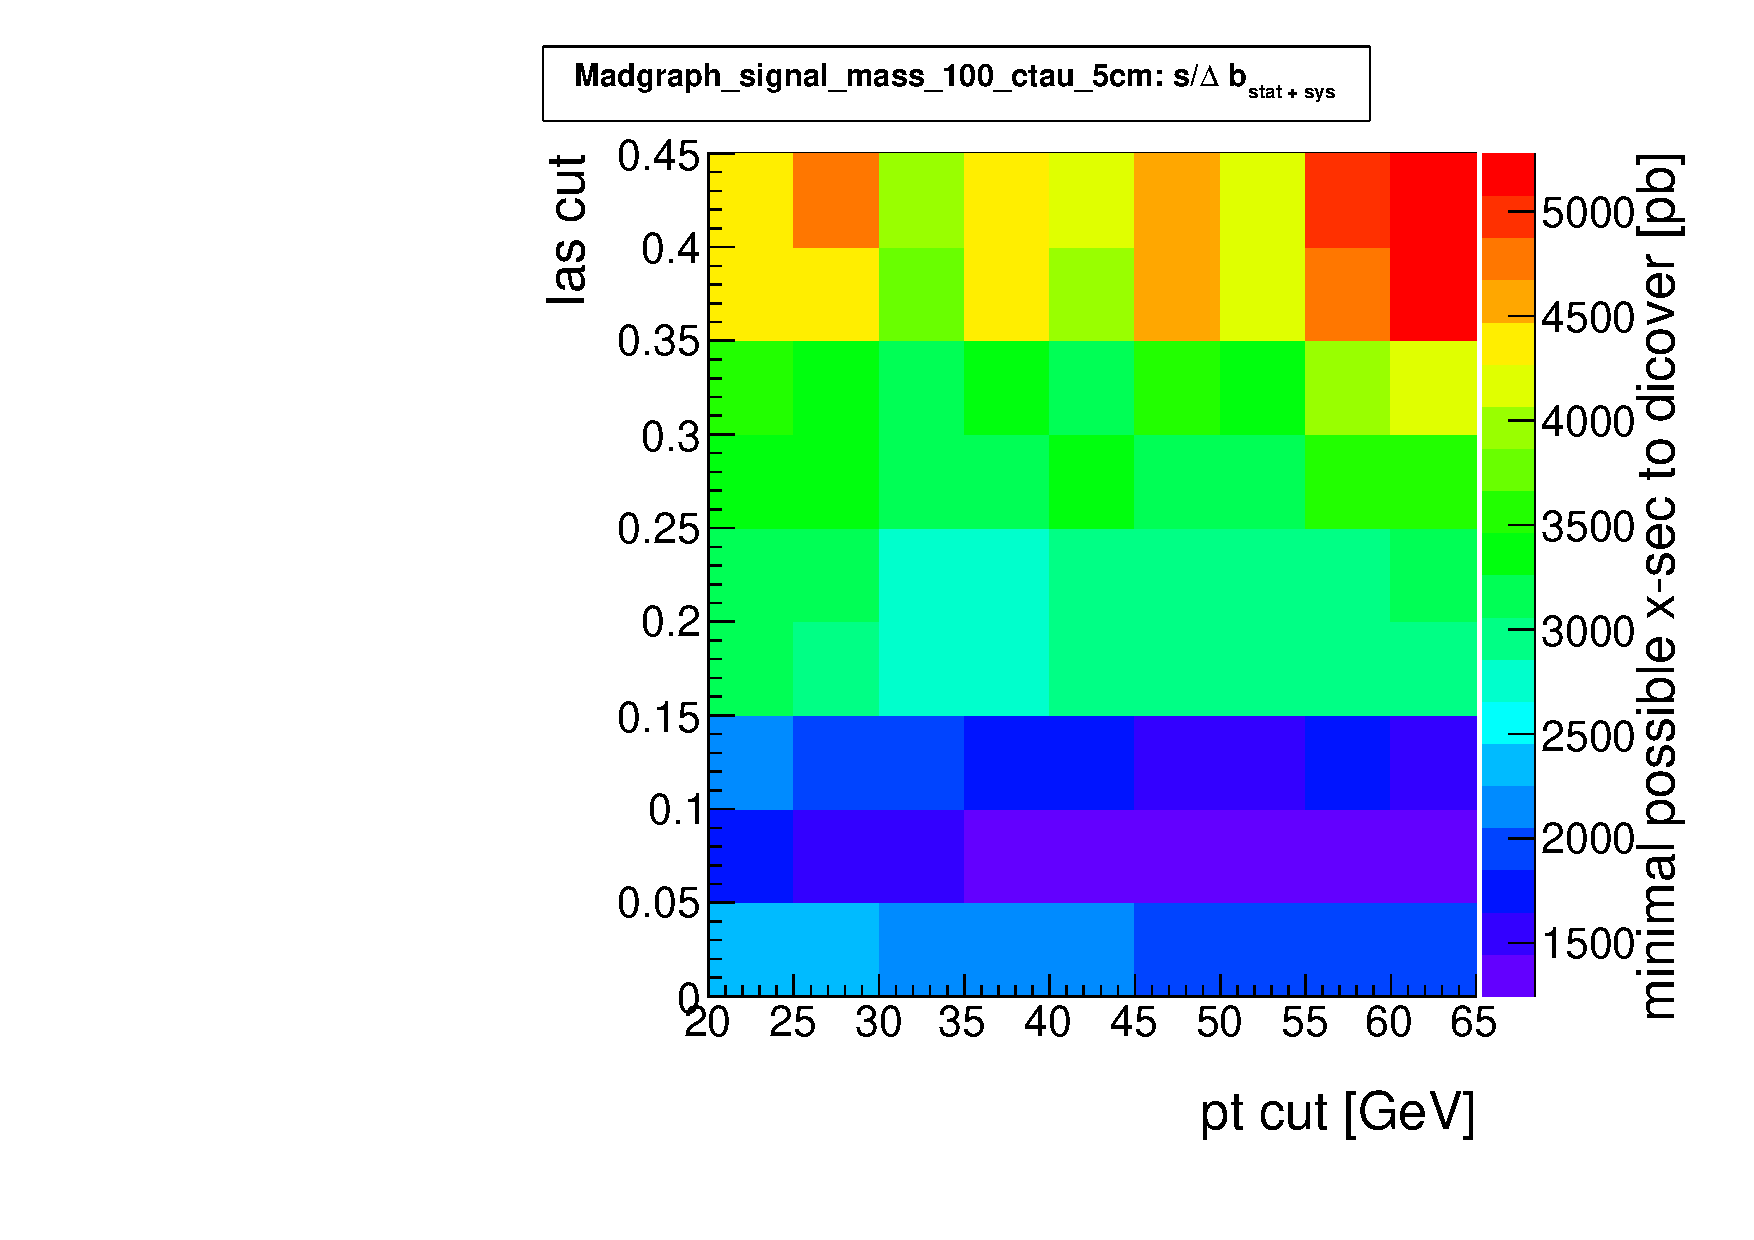
\includegraphics[width=0.49\textwidth]{figures/analysis/Optimisation/Madgraph_signal_mass_100_ctau_5cm_ECaloLe5_SOverDeltaBStatPlusSys.pdf} 
    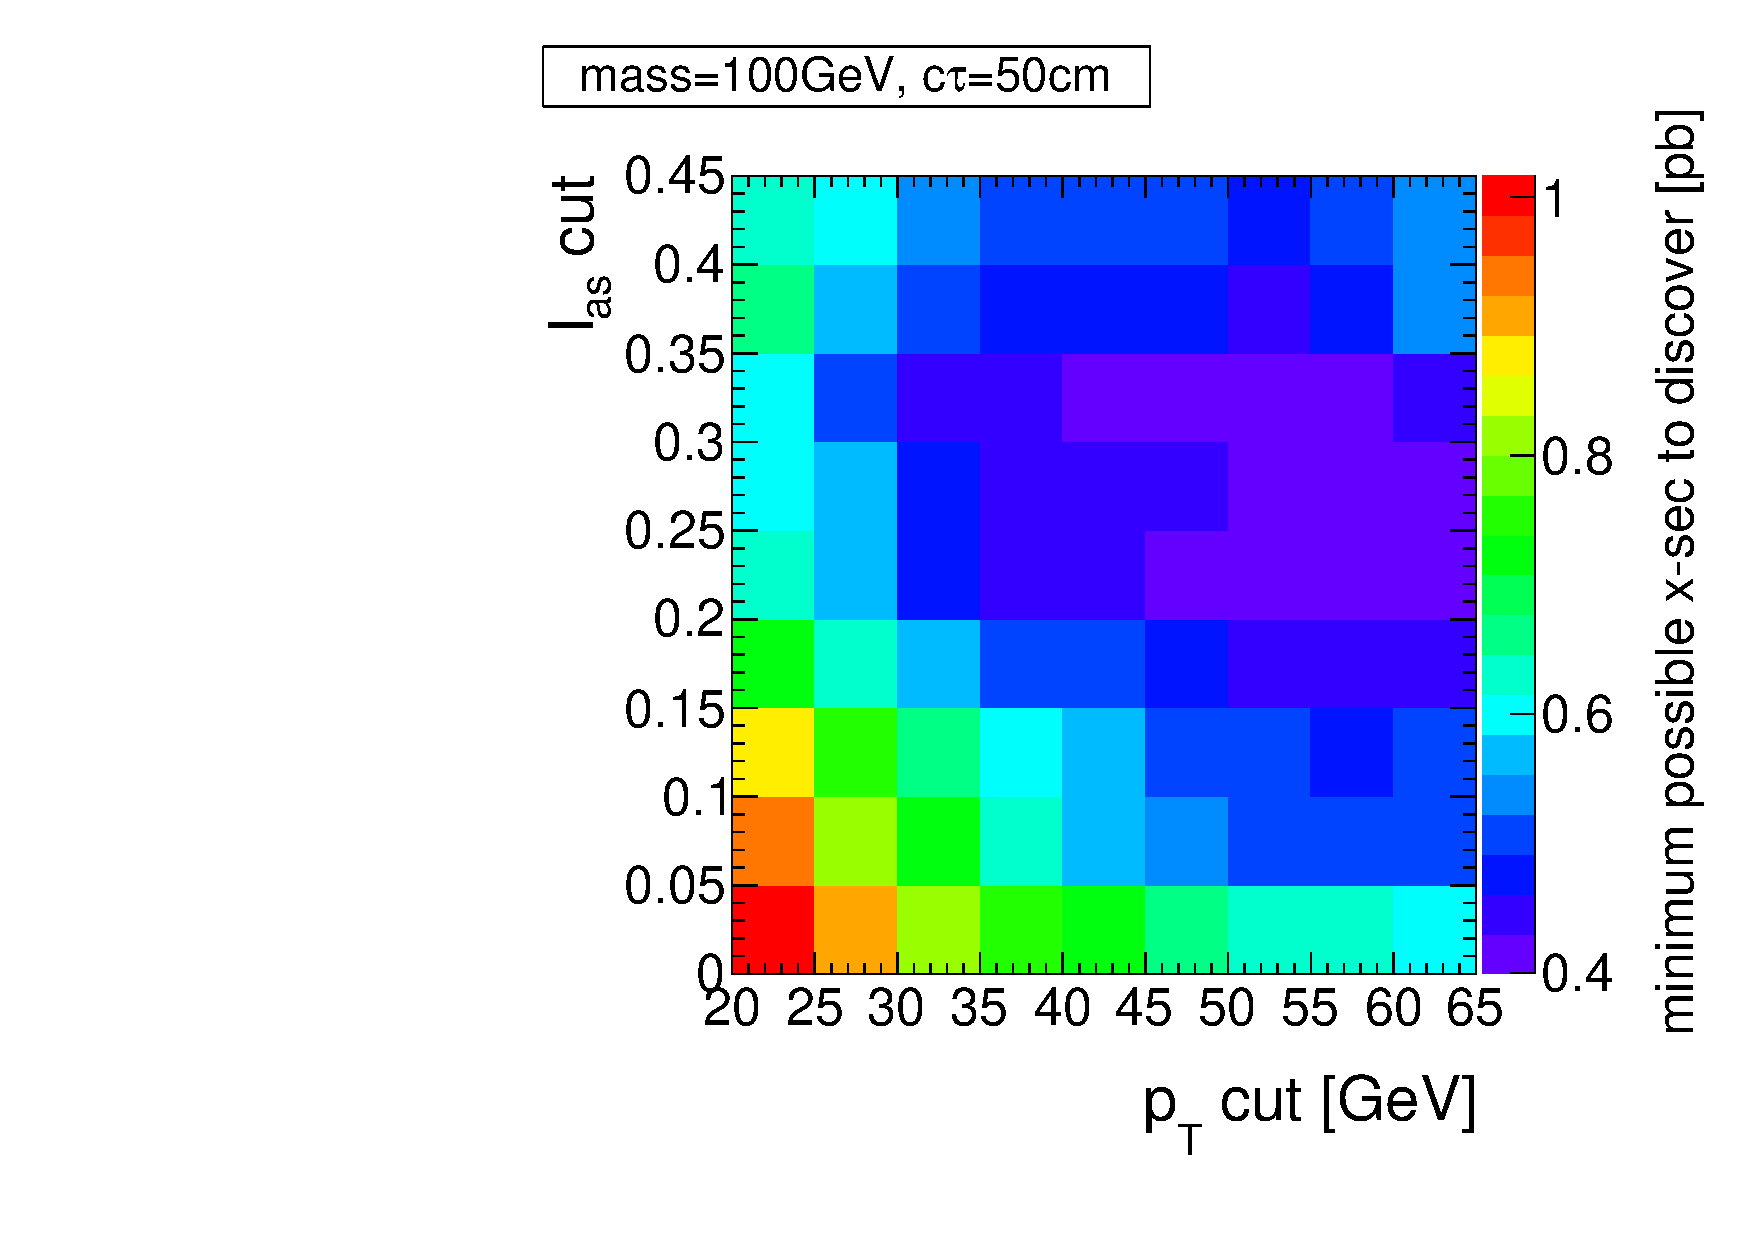
\includegraphics[width=0.49\textwidth]{figures/analysis/Optimisation/Madgraph_signal_mass_100_ctau_50cm_ECaloLe5_SOverDeltaBStatPlusSys.pdf}\\ 
    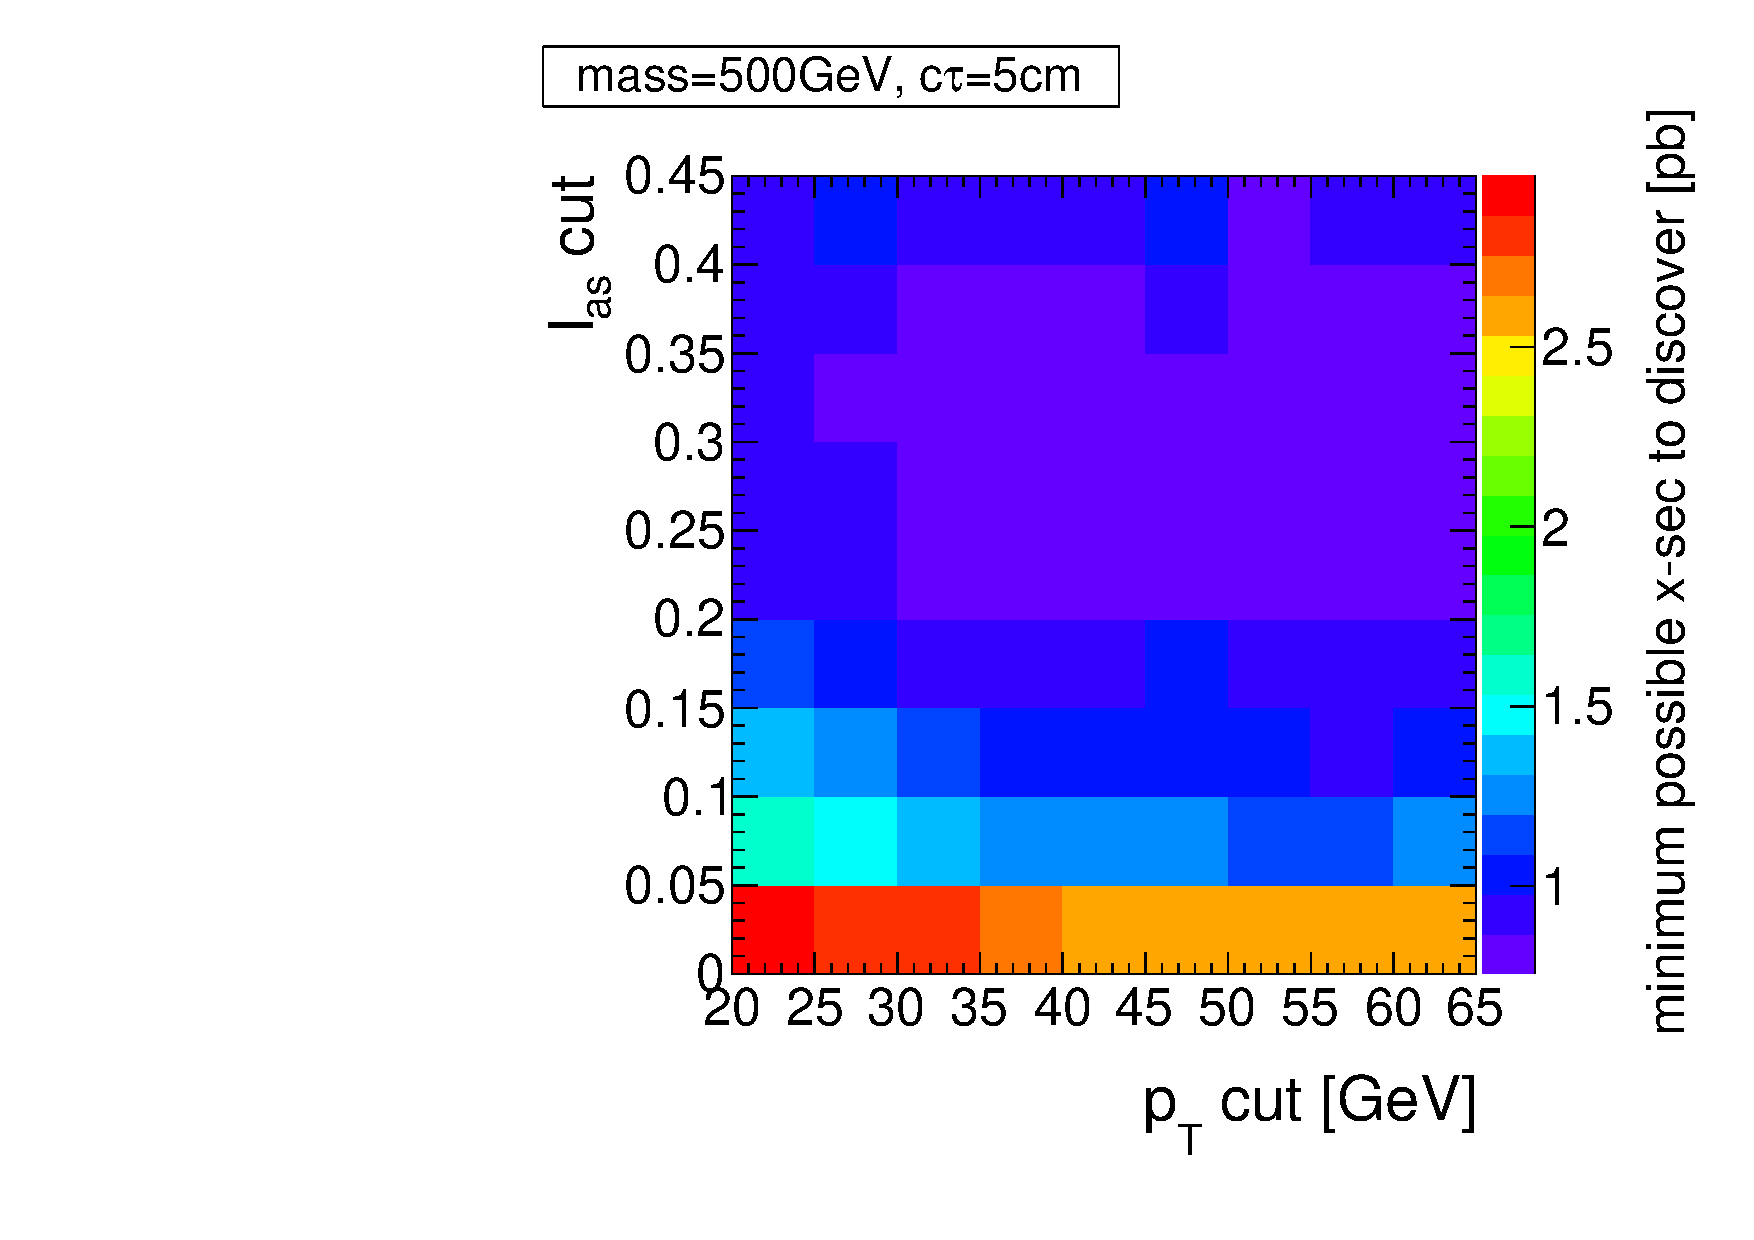
\includegraphics[width=0.49\textwidth]{figures/analysis/Optimisation/Madgraph_signal_mass_500_ctau_5cm_ECaloLe5_SOverDeltaBStatPlusSys.pdf}
    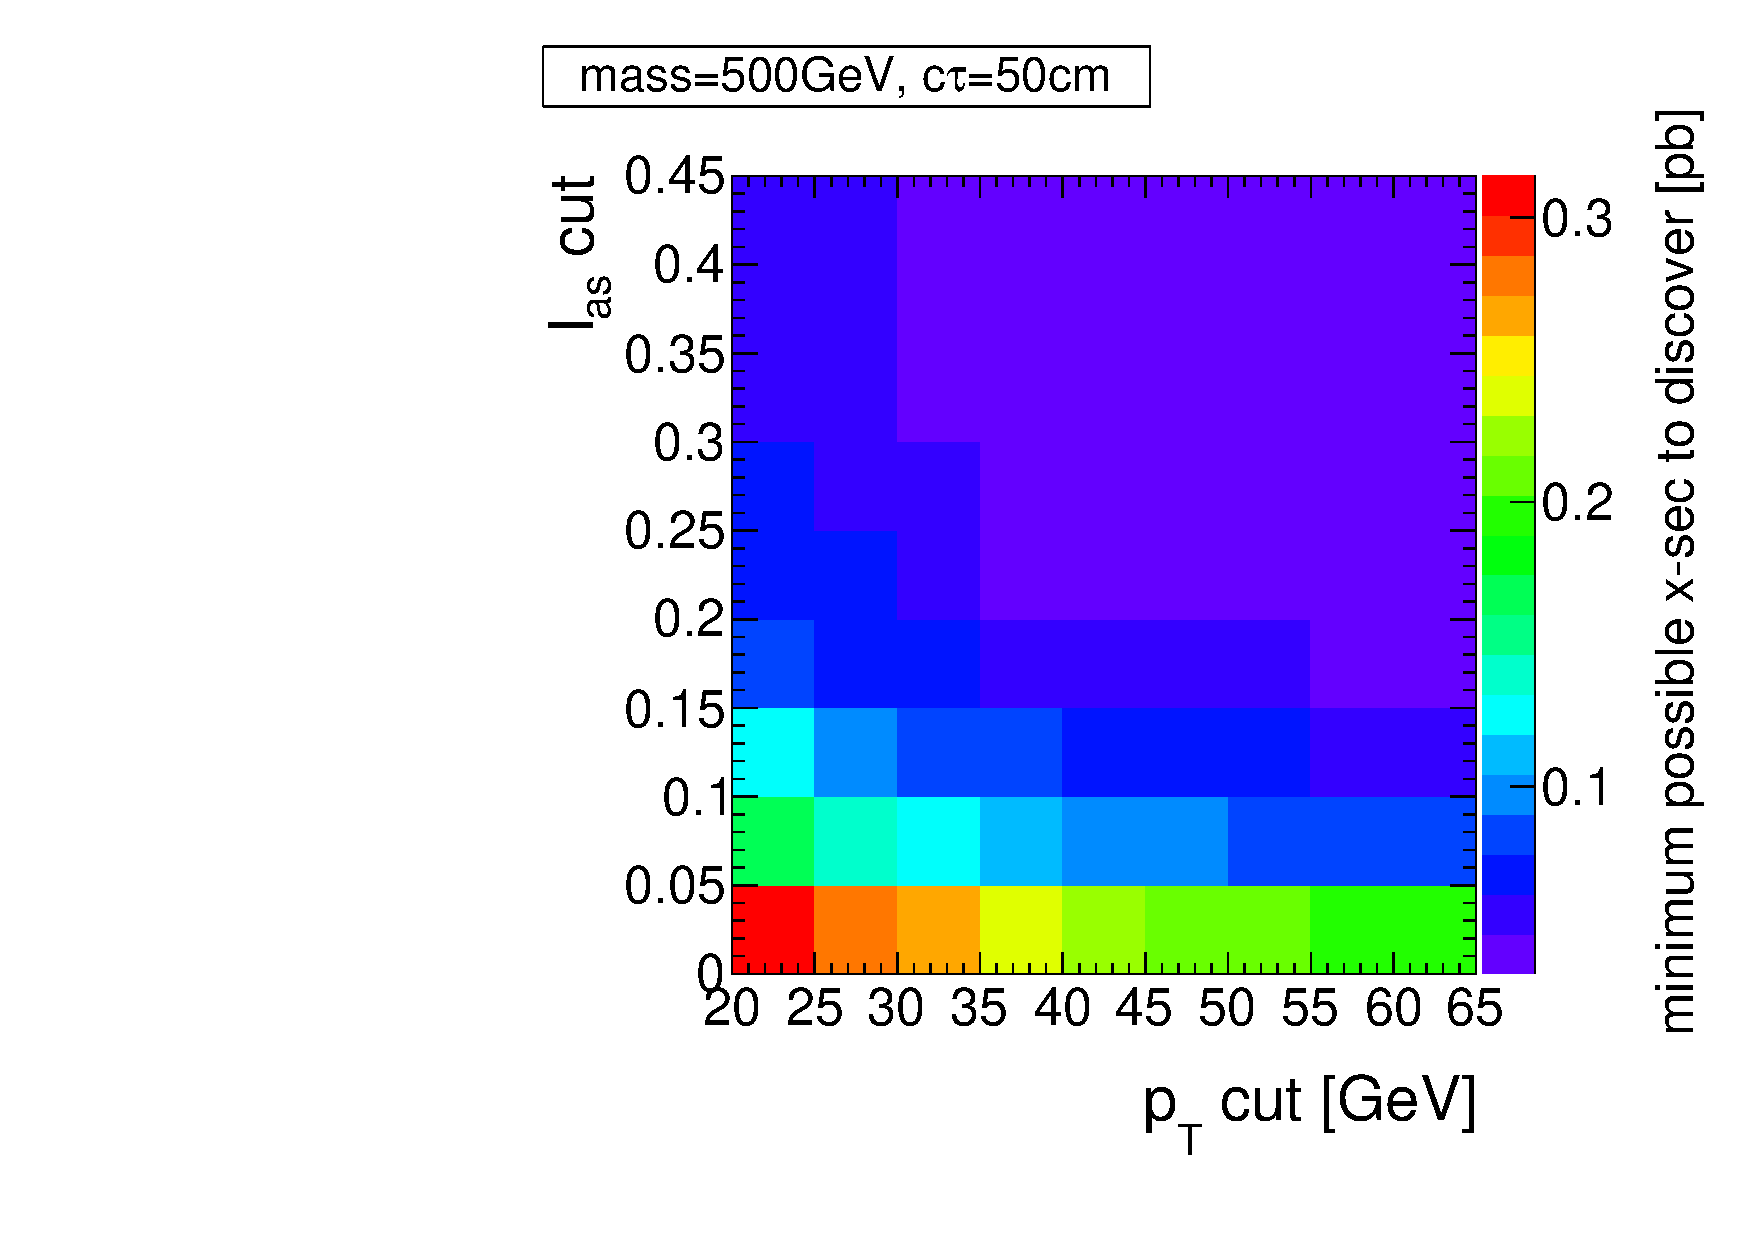
\includegraphics[width=0.49\textwidth]{figures/analysis/Optimisation/Madgraph_signal_mass_500_ctau_50cm_ECaloLe5_SOverDeltaBStatPlusSys.pdf} 
  \end{tabular}
  \caption{Minimum possible cross section that can be discovered with 5$\sigma$ significance as a function of minimum \pt and \ias requirements for four different signal models.
           The systematic uncertainties are taken to be 20\% and 100\% for the fake and the leptonic background respectively.
           The uncertainty on the background arising from the limited size of the used samples are propagated consistently to the search optimisation.
           In Table~\ref{fig:optimisationApp} of Appendix~\ref{app:OptimisationApp}, the corresponding histograms of the background yield, the background uncertainty and the signal yield for the four signal models can be found.}
  \vspace{10pt}
  \label{fig:optimisation}
\end{figure}
Similar to the full optimisation, it can be seen that for low masses and low lifetimes, the highest search sensitivity is achieved by imposing rather soft selection cuts on \ias and \pt.
Optimising for higher lifetime pushes the optimal selection in \pt and \ias to larger values, where signal models with higher masses prefer even tighter \ias selection cuts than the corresponding lower mass signal model.
It can also be seen, that for low lifetimes, the \pt dependence of the search sensitivity is less pronounced than for long lifetimes.\\


Based on the optimisation, four different exclusive signal regions are defined in order to achieve an optimal coverage over a wide mass space and a high sensitivity for different lifetimes:
\begin{enumerate}[1.)]
\item $30\gev<\pt<50\gev$ and $0.05<\ias<0.3$
\item $\pt>50\gev$ and $0.05<\ias<0.3$
\item $30\gev<\pt<50\gev$ and $\ias>0.3$
\item $\pt>50\gev$ and $\ias>0.3$.
\end{enumerate}

%The unblinded results of the search for highly ionising, short tracks are presented in the following chapter.
%%%%%%%%%%%%%%%%%%%%%%%%%%%%%%%%%%%%%%%%%%%%%%%%%%%%%%%%%%%%%%%%%%%%%%%%%%%%%%%%%%%%%%%%%%%%%%%%%%%%%%%%%%%%%%%%%%%%%%%%%%%%%%%%%%%%%%%%%%%%%%%%%%%%%%%%%%%%%%%%%%%%%%%
%%%%%%%%%%%%%%%%%%%%%%%%%%%%%%%%%%%%%%%%%%%%%%%%%%%%%%%%%%%%%%%%%%%%%%%%%%%%%%%%%%%%%%%%%%%%%%%%%%%%%%%%%%%%%%%%%%%%%%%%%%%%%%%%%%%%%%%%%%%%%%%%%%%%%%%%%%%%%%%%%%%%%%%

